\documentclass[tikz,border=5pt]{standalone}
\usepackage[T1]{fontenc}
\usepackage{lmodern,amsmath,amssymb}
\usetikzlibrary{arrows.meta,calc,positioning,fit,backgrounds,shapes.geometric,matrix,decorations.pathreplacing,patterns}
\definecolor{ink}{gray}{0.08}
\definecolor{wash}{gray}{0.965}
\definecolor{soft}{gray}{0.45}
\tikzset{box/.style={draw=ink,line width=.65pt,fill=white,align=center,inner sep=4pt,outer sep=0pt,font=\small},flow/.style={draw=ink,line width=.65pt,-{Latex[length=1.8mm,width=1.3mm]},rounded corners=2pt},annotation/.style={font=\scriptsize,text=soft,align=center},groupbox/.style={draw=soft,dashed,line width=.45pt,fill=wash}}
\begin{document}
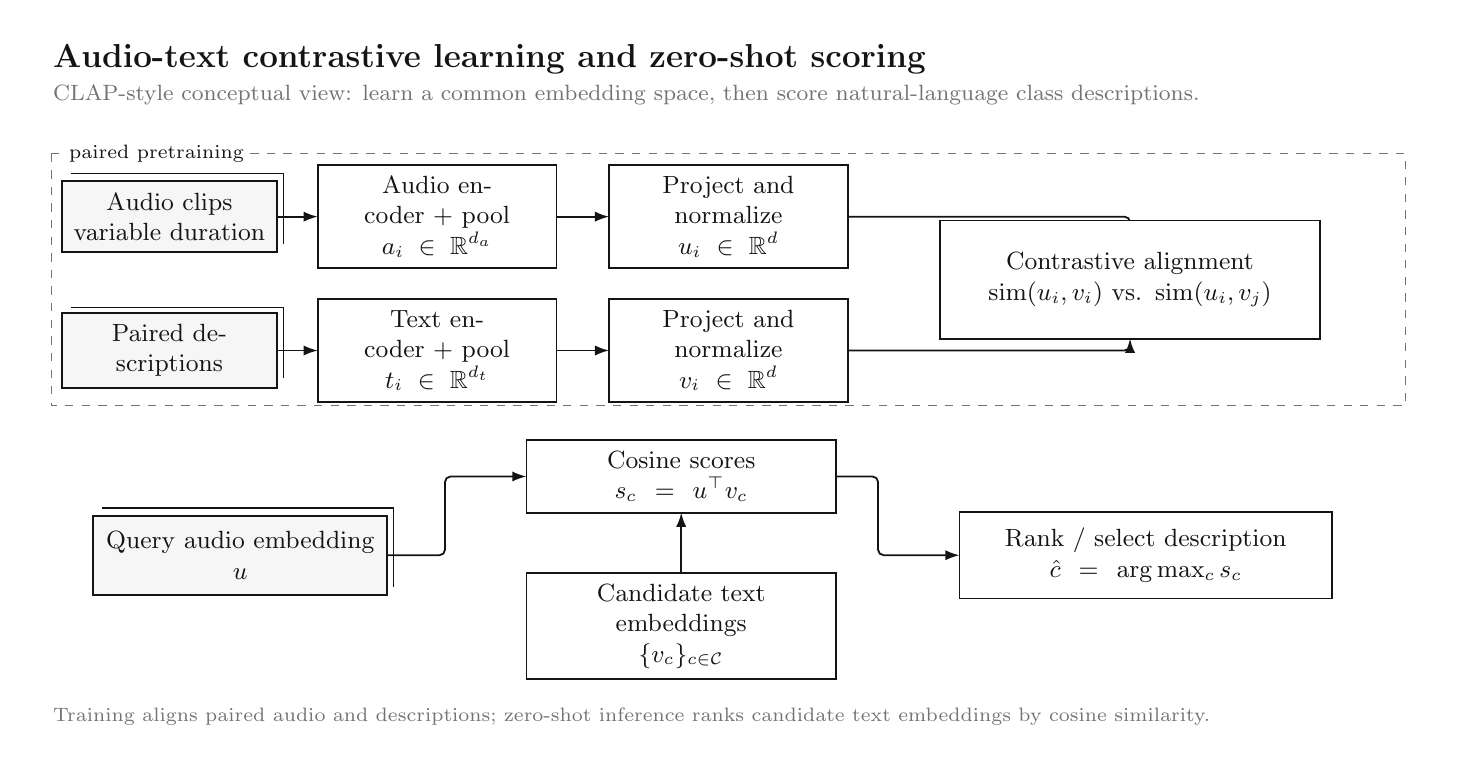
\begin{tikzpicture}[x=1cm,y=-1cm,font=\rmfamily,text=ink]

\path[use as bounding box] (0,0) rectangle (18,9);
\node[anchor=west,font=\large\bfseries] at (.2,.4) {Audio-text contrastive learning and zero-shot scoring};
\node[anchor=west,font=\footnotesize,text=soft] at (.2,.85) {CLAP-style conceptual view: learn a common embedding space, then score natural-language class descriptions.};
\begin{pgfonlayer}{background}
\end{pgfonlayer}
\node[box,fill=wash,minimum width=2.7cm,minimum height=0.9cm,text width=2.45cm] (audio) at (1.8,2.4) {Audio clips\\variable duration};
\draw[ink,line width=.4pt] (0.5499999999999999,1.8499999999999999) -- (3.2500000000000004,1.8499999999999999) -- (3.2500000000000004,2.75);
\node[box,minimum width=3.0cm,minimum height=1.0cm,text width=2.75cm] (aenc) at (5.2,2.4) {Audio encoder + pool\\$a_i\in\mathbb{R}^{d_a}$};
\node[box,minimum width=3.0cm,minimum height=1.0cm,text width=2.75cm] (aproj) at (8.9,2.4) {Project and normalize\\$u_i\in\mathbb{R}^{d}$};
\node[box,fill=wash,minimum width=2.7cm,minimum height=0.9cm,text width=2.45cm] (desc) at (1.8,4.1) {Paired descriptions};
\draw[ink,line width=.4pt] (0.5499999999999999,3.5499999999999994) -- (3.2500000000000004,3.5499999999999994) -- (3.2500000000000004,4.45);
\node[box,minimum width=3.0cm,minimum height=1.0cm,text width=2.75cm] (tenc) at (5.2,4.1) {Text encoder + pool\\$t_i\in\mathbb{R}^{d_t}$};
\node[box,minimum width=3.0cm,minimum height=1.0cm,text width=2.75cm] (tproj) at (8.9,4.1) {Project and normalize\\$v_i\in\mathbb{R}^{d}$};
\node[box,minimum width=4.8cm,minimum height=1.5cm,text width=4.55cm] (align) at (14.0,3.2) {Contrastive alignment\\$\mathrm{sim}(u_i,v_i)$ vs. $\mathrm{sim}(u_i,v_j)$};
\node[box,fill=wash,minimum width=3.7cm,minimum height=1.0cm,text width=3.45cm] (query) at (2.7,6.7) {Query audio embedding\\$u$};
\draw[ink,line width=.4pt] (0.9500000000000001,6.1000000000000005) -- (4.65,6.1000000000000005) -- (4.65,7.1000000000000005);
\node[box,minimum width=3.9cm,minimum height=0.9cm,text width=3.65cm] (candidates) at (8.3,7.6) {Candidate text embeddings\\$\{v_c\}_{c\in\mathcal C}$};
\node[box,minimum width=3.9cm,minimum height=0.9cm,text width=3.65cm] (score) at (8.3,5.7) {Cosine scores\\$s_c=u^{\top}v_c$};
\node[box,minimum width=4.7cm,minimum height=1.1cm,text width=4.45cm] (rank) at (14.2,6.7) {Rank / select description\\$\hat c=\arg\max_c s_c$};
\begin{pgfonlayer}{background}
\draw[flow] (audio.east) -- (aenc.west);
\draw[flow] (aenc.east) -- (aproj.west);
\draw[flow] (desc.east) -- (tenc.west);
\draw[flow] (tenc.east) -- (tproj.west);
\draw[flow] (aproj.east) -- (14.0,2.4) -- (align.north);
\draw[flow] (tproj.east) -- (14.0,4.1) -- (align.south);
\draw[flow] (query.east) -- (5.3,6.7) -- (5.3,5.7) -- (score.west);
\draw[flow] (candidates.north) -- (score.south);
\draw[flow] (score.east) -- (10.8,5.7) -- (10.8,6.7) -- (rank.west);
\end{pgfonlayer}
\draw[draw=soft,dashed,line width=.45pt] (0.3,1.6) rectangle (17.5,4.800000000000001);
\node[anchor=west,font=\scriptsize,fill=white,inner sep=2pt] at (0.44999999999999996,1.6) {paired pretraining};
\node[anchor=west,align=left,font=\scriptsize,text=soft,text width=17.6cm] at (.2,8.75) {Training aligns paired audio and descriptions; zero-shot inference ranks candidate text embeddings by cosine similarity.};
\end{tikzpicture}
\end{document}
